\documentclass[12pt,a4paper]{article}
\usepackage[utf8]{vietnam}
\usepackage{amsmath,amssymb}
\usepackage{tabularx}
\usepackage{tikz}
\usetikzlibrary{calc,angles,quotes,arrows.meta,patterns}
\usepackage{xcolor}
\usepackage{enumitem}
\usepackage{fancyhdr}
\usepackage[top=1.2cm, bottom=1.2cm, left=1.5cm, right=1.5cm]{geometry}
\usepackage[loigiai]{ex_test}
\SAOPTN{widthSA=2.6,heightSA=0.62}

\setlength{\headheight}{15pt}
\setlength{\parskip}{0pt}

\pagestyle{fancy}
\fancyhf{}
\rhead{\textit{Môn Toán 6 -- Hướng dẫn giải Đề số 4}}
\lhead{\textit{Bộ đề ôn tập Giữa học kì I}}
\cfoot{\thepage}

\begin{document}

\begin{center}
  \textbf{\Large HƯỚNG DẪN GIẢI CHI TIẾT VÀ BẢNG ĐÁP ÁN}\\
  \textbf{\large ĐỀ ÔN TẬP GIỮA HỌC KỲ I -- ĐỀ SỐ 4}\\
  \textit{Môn: Toán 6 -- Năm học 2026 -- 2027}
\end{center}
\vspace{2mm}

% --- BẢNG ĐÁP ÁN TRẮC NGHIỆM TỔNG HỢP ---
\noindent\textbf{\large A. BẢNG ĐÁP ÁN TRẮC NGHIỆM TỔNG HỢP}
\vspace{1.5mm}

\noindent\textbf{1. Phần I (Mỗi câu trả lời đúng được 0,25 điểm):}
\begin{center}
\begin{tabular}{|c|c|c|c|c|c|c|c|c|c|c|c|c|}
\hline
\textbf{Câu} & \textbf{1} & \textbf{2} & \textbf{3} & \textbf{4} & \textbf{5} & \textbf{6} & \textbf{7} & \textbf{8} & \textbf{9} & \textbf{10} & \textbf{11} & \textbf{12} \\
\hline
\textbf{Đ/A} & \textbf{C} & \textbf{D} & \textbf{C} & \textbf{D} & \textbf{A} & \textbf{C} & \textbf{B} & \textbf{B} & \textbf{D} & \textbf{B} & \textbf{A} & \textbf{B} \\
\hline
\end{tabular}
\end{center}
\vspace{1mm}

\noindent\textbf{2. Phần II (Đúng/Sai):}
\begin{center}
\begin{tabular}{|c|c|c|c|c||c|c|c|c|c|}
\hline
\textbf{Câu 1} & \textbf{a)} & \textbf{b)} & \textbf{c)} & \textbf{d)} & \textbf{Câu 2} & \textbf{a)} & \textbf{b)} & \textbf{c)} & \textbf{d)} \\
\hline
\textbf{Đ/S} & \textbf{Đ} & \textbf{S} & \textbf{Đ} & \textbf{Đ} & \textbf{Đ/S} & \textbf{Đ} & \textbf{Đ} & \textbf{Đ} & \textbf{Đ} \\
\hline
\end{tabular}
\end{center}
\vspace{1mm}

\noindent\textbf{3. Phần III (Mỗi câu trả lời đúng được 1,0 điểm):}
\begin{center}
\begin{tabular}{|c|c|c|}
\hline
\textbf{Câu} & \textbf{Câu 1} & \textbf{Câu 2} \\
\hline
\textbf{Đáp án} & \textbf{10} & \textbf{$x$ là số chẵn} \\
\hline
\end{tabular}
\end{center}
\vspace{3mm}

% --- LỜI GIẢI CHI TIẾT ---
\noindent\textbf{\large B. HƯỚNG DẪN GIẢI CHI TIẾT TỪNG CÂU}
\vspace{2mm}

\noindent\textbf{\large PHẦN I. CÂU TRẮC NGHIỆM NHIỀU PHƯƠNG ÁN LỰA CHỌN}
\vspace{1mm}
\begin{ex}
Chữ số $5$ trong số tự nhiên $2358$ có giá trị là:
\choice
{$5000$}
{$500$}
{\True $50$}
{$5$}
\loigiai{
Trong số tự nhiên $2358$, chữ số 5 nằm ở hàng chục nên có giá trị là $5 \times 10 = 50$.
}
\end{ex}

\begin{ex}
Số $19$ trong hệ La Mã được viết là:
\choice
{IX}
{IXX}
{XXI}
{\True XIX}
\loigiai{
Số $19 = 10 + 9$, trong đó 10 là $\mathrm{X}$ và 9 là $\mathrm{IX}$, do đó số 19 được viết là $\mathrm{XIX}$.
}
\end{ex}

\begin{ex}
Tích $2 \cdot 2 \cdot 2 \cdot 2 \cdot 2 \cdot 2$ được viết gọn dưới dạng một lũy thừa là:
\choice
{$2^2$}
{$6^2$}
{\True $2^6$}
{$5^2$}
\loigiai{
Tích của 6 thừa số 2 bằng nhau được viết gọn là $2^6$.
}
\end{ex}

\begin{ex}
Khẳng định nào dưới đây là đúng?
\choice
{Hợp số là số chỉ có hai ước là 1 và chính nó}
{Hợp số là số tự nhiên có đúng hai ước}
{Số nguyên tố là số tự nhiên lớn hơn 1 có nhiều hơn hai ước}
{\True Số nguyên tố là số tự nhiên lớn hơn 1, chỉ có hai ước là 1 và chính nó}
\loigiai{
Theo định nghĩa SGK: Số nguyên tố là số tự nhiên lớn hơn 1, chỉ có hai ước là 1 và chính nó.
}
\end{ex}

\begin{ex}
Trong một hình vuông, một đường chéo có độ dài $8\text{ cm}$. Khi đó độ dài đường chéo còn lại là:
\choice
{\True $8\text{ cm}$}
{$4\text{ cm}$}
{$16\text{ cm}$}
{$32\text{ cm}$}
\loigiai{
Hình vuông có hai đường chéo bằng nhau, do đó đường chéo còn lại cũng có độ dài bằng $8\text{ cm}$.
}
\end{ex}

\begin{ex}
Số $75$ được phân tích ra thừa số nguyên tố là:
\choice
{$2 \cdot 3 \cdot 5$}
{$3 \cdot 5 \cdot 7$}
{\True $3 \cdot 5^2$}
{$3^2 \cdot 5$}
\loigiai{
Ta có: $75 = 3 \cdot 25 = 3 \cdot 5^2$.
}
\end{ex}

\begin{ex}
Hình có bốn góc bằng nhau và bốn cạnh bằng nhau là hình gì?
\choice
{Hình chữ nhật}
{\True Hình vuông}
{Hình bình hành}
{Hình thoi}
\loigiai{
Hình vuông là hình có bốn cạnh bằng nhau và bốn góc bằng nhau (đều là góc vuông $90^\circ$).
}
\end{ex}

\begin{ex}
Thứ tự thực hiện các phép tính đối với biểu thức không có dấu ngoặc là:
\choice
{Nhân và chia $\to$ Lũy thừa $\to$ Cộng và trừ}
{\True Lũy thừa $\to$ Nhân và chia $\to$ Cộng và trừ}
{Cộng và trừ $\to$ Nhân và chia $\to$ Lũy thừa}
{Lũy thừa $\to$ Cộng và trừ $\to$ Nhân và chia}
\loigiai{
Thứ tự chuẩn khi thực hiện phép tính không có ngoặc là: Lũy thừa $\to$ Nhân và chia $\to$ Cộng và trừ.
}
\end{ex}

\begin{ex}
Trong các dãy số sau, dãy nào được sắp xếp theo thứ tự tăng dần đúng?
\choice
{$0; -20; -15; -12; 8$}
{$-15; -12; -20; 0; 8$}
{$8; 0; -12; -15; -20$}
{\True $-20; -15; -12; 0; 8$}
\loigiai{
So sánh các số nguyên ta có: $-20 < -15 < -12 < 0 < 8$. Do đó dãy sắp xếp tăng dần đúng là D.
}
\end{ex}

\begin{ex}
\immini{
Cho hình vẽ bên. Phát biểu nào dưới đây là đúng?
\choice
{$ABCD$ là hình thoi}
{\True $ABCD$ là hình bình hành}
{$ABCE$ là hình thang cân}
{$ABCE$ là hình chữ nhật}
}{
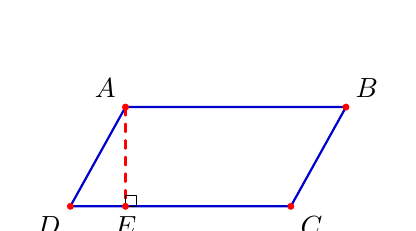
\begin{tikzpicture}[scale=0.7, baseline=(current bounding box.center), line cap=round, line join=round]
  \coordinate (D) at (0,0); \coordinate (E) at (1,0); \coordinate (C) at (4,0);
  \coordinate (A) at (1,1.8); \coordinate (B) at (5,1.8);
  \draw[thick, blue!80!black] (D) -- (C) -- (B) -- (A) -- cycle;
  \draw[thick, dashed, red] (A) -- (E);
  \draw (E) rectangle +(0.2,0.2);
  \foreach \p in {A,B,C,D,E} \fill[red] (\p) circle (1.8pt);
  \node[above left] at (A) {$A$}; \node[above right] at (B) {$B$};
  \node[below right] at (C) {$C$}; \node[below left] at (D) {$D$}; \node[below] at (E) {$E$};
\end{tikzpicture}
}
\loigiai{
Tứ giác $ABCD$ có các cặp cạnh đối song song và bằng nhau ($AB \parallel CD, AD \parallel BC$) nên $ABCD$ là hình bình hành.
}
\end{ex}

\begin{ex}
Trong một tam giác đều, mỗi góc có số đo bằng:
\choice
{\True $60^\circ$}
{$45^\circ$}
{$90^\circ$}
{$30^\circ$}
\loigiai{
Tam giác đều có ba góc bằng nhau và mỗi góc có số đo bằng $60^\circ$.
}
\end{ex}

\begin{ex}
\immini{
Cho hình thoi $ABCD$ như hình vẽ bên. Khẳng định nào sau đây là đúng?
\choice
{Bốn cạnh của hình thoi không bằng nhau}
{\True Hình thoi $ABCD$ có hai đường chéo vuông góc với nhau}
{Hình thoi $ABCD$ có cạnh $AB$ song song với cạnh $AD$}
{Hình thoi $ABCD$ có bốn góc vuông}
}{
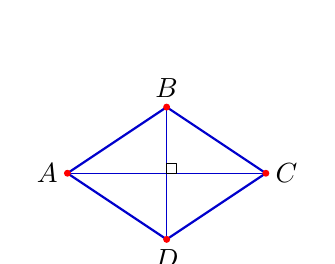
\begin{tikzpicture}[scale=0.7, baseline=(current bounding box.center), line cap=round, line join=round]
  \coordinate (A) at (-1.8,0); \coordinate (B) at (0,1.2);
  \coordinate (C) at (1.8,0); \coordinate (D) at (0,-1.2);
  \draw[thick, blue!80!black] (A) -- (B) -- (C) -- (D) -- cycle;
  \draw[blue!80!black] (A) -- (C); \draw[blue!80!black] (B) -- (D);
  \draw (0,0) rectangle +(0.18,0.18);
  \foreach \p in {A,B,C,D} \fill[red] (\p) circle (1.8pt);
  \node[left] at (A) {$A$}; \node[above] at (B) {$B$};
  \node[right] at (C) {$C$}; \node[below] at (D) {$D$};
\end{tikzpicture}
}
\loigiai{
Một trong những tính chất đặc trưng của hình thoi là hai đường chéo vuông góc với nhau tại trung điểm của mỗi đường.
}
\end{ex}


\setcounter{ex}{0}
\noindent\textbf{\large PHẦN II. CÂU TRẮC NGHIỆM ĐÚNG SAI}
\vspace{1mm}
\begin{ex}
Trong $15$ số tự nhiên đầu tiên (từ $0$ đến $14$), các khẳng định sau đây đúng hay sai?
\choiceTF
{\True Trong các số đã cho, có $2$ số chia hết cho cả $2$ và $5$}
{Trong các số đã cho, có $5$ số chia hết cho $9$}
{\True Trong các số đã cho, có $6$ số là số nguyên tố}
{\True Trong các số đã cho, có $5$ số là bội của $3$}
\loigiai{
\begin{itemize}[leftmargin=0.6cm, itemsep=1pt]
\item \textbf{a)} \textbf{Đúng}. Các số có tận cùng bằng 0 từ 0 đến 14 gồm: $\{0; 10\}$ (đúng 2 số). Khẳng định đúng.
\item \textbf{b)} \textbf{Sai}. Các số chia hết cho 9 từ 0 đến 14 gồm: $\{0; 9\}$ (chỉ có 2 số). Khẳng định sai.
\item \textbf{c)} \textbf{Đúng}. Các số nguyên tố từ 0 đến 14 gồm: $\{2; 3; 5; 7; 11; 13\}$ (đúng 6 số). Khẳng định đúng.
\item \textbf{d)} \textbf{Đúng}. Các bội của 3 từ 0 đến 14 gồm: $\{0; 3; 6; 9; 12\}$ (đúng 5 số). Khẳng định đúng.
\end{itemize}
}
\end{ex}

\begin{ex}
Cho các hình sau: tam giác đều, hình vuông, lục giác đều, hình chữ nhật, hình thoi, hình bình hành, hình thang cân. Các khẳng định sau đây đúng hay sai?
\choiceTF
{\True Hình tam giác đều, hình vuông, hình lục giác đều có tất cả các cạnh bằng nhau}
{\True Có $2$ hình có hai đường chéo vuông góc với nhau}
{\True Có $3$ hình có hai cạnh đối song song và các đường chéo bằng nhau}
{\True Hình lục giác đều có độ dài đường chéo chính gấp đôi độ dài cạnh}
\loigiai{
\begin{itemize}[leftmargin=0.6cm, itemsep=1pt]
\item \textbf{a)} \textbf{Đúng}. Các đa giác đều luôn có tất cả các cạnh bằng nhau. Khẳng định đúng.
\item \textbf{b)} \textbf{Đúng}. Hai hình có đường chéo vuông góc là hình vuông và hình thoi. Khẳng định đúng.
\item \textbf{c)} \textbf{Đúng}. Ba hình có hai cạnh đối song song và đường chéo bằng nhau là: hình chữ nhật, hình vuông và hình thang cân. Khẳng định đúng.
\item \textbf{d)} \textbf{Đúng}. Đường chéo chính của lục giác đều bằng 2 lần cạnh tam giác đều cấu thành. Khẳng định đúng.
\end{itemize}
}
\end{ex}


\setcounter{ex}{0}
\noindent\textbf{\large PHẦN III. CÂU HỎI TRẢ LỜI NGẮN}
\vspace{1mm}
\begin{ex}
Một hình chữ nhật có diện tích là $120\text{ cm}^2$ và có chiều dài là $12\text{ cm}$. Tính độ dài chiều rộng của hình chữ nhật đó (đơn vị: cm). \shortans{$10$}
\loigiai{
Chiều rộng của hình chữ nhật là: $120 : 12 = 10\text{ (cm)}$.
}
\end{ex}

\begin{ex}
Cho $x$ là số tự nhiên. Để biểu thức $A = 12 + 14 + x$ chia hết cho $2$ thì điều kiện của $x$ là gì? \shortans{$x$ là số chẵn}
\loigiai{
Vì $12 \ \vdots \ 2$ và $14 \ \vdots \ 2$ nên $(12 + 14) \ \vdots \ 2$. Để tổng $A = (12 + 14) + x \ \vdots \ 2$ thì $x$ phải chia hết cho 2, tức là $x$ là số tự nhiên chẵn.
}
\end{ex}


\setcounter{ex}{0}
\noindent\textbf{\large PHẦN IV. TỰ LUẬN (3,0 ĐIỂM - CÓ BAREM ĐIỂM CHI TIẾT)}
\vspace{1mm}
\begin{ex} (1.0 điểm)
Thực hiện phép tính:
\begin{enumerate}[label=\textbf{\alph*)}, leftmargin=0.8cm, itemsep=2pt]
\item $36 - 36 : 6 + 24$
\item $2 \cdot 3^2 - 24 : (3 \cdot 2^2)$
\end{enumerate}
\loigiai{
\begin{itemize}[leftmargin=0.5cm, itemsep=3pt]
\item \textbf{a)} $36 - 36 : 6 + 24 = 36 - 6 + 24 = 30 + 24 = 54$. \hfill \textbf{[0.5đ]}
\item \textbf{b)} $2 \cdot 3^2 - 24 : (3 \cdot 2^2) = 2 \cdot 9 - 24 : (3 \cdot 4) = 18 - 24 : 12 = 18 - 2 = 16$. \hfill \textbf{[0.5đ]}
\end{itemize}
}
\end{ex}
\vspace{1.5mm}

\begin{ex} (0.75 điểm)
\begin{enumerate}[label=\textbf{\alph*)}, leftmargin=0.8cm, itemsep=2pt]
\item Học sinh lớp 6C khi xếp thành hàng 4, hàng 5, hàng 8 đều vừa đủ hàng. Hỏi số học sinh của lớp 6C là bao nhiêu, biết rằng số học sinh của lớp 6C nhỏ hơn 45?
\end{enumerate}
\loigiai{
\begin{itemize}[leftmargin=0.5cm, itemsep=3pt]
\item \textbf{a)} Gọi số học sinh của lớp 6C là $a$ ($a \in \mathbb{N}^*$ và $a < 45$).\
Vì khi xếp hàng 4, hàng 5, hàng 8 đều vừa đủ nên $a \in \text{BC}(4, 5, 8)$.\
Ta có: $4 = 2^2$; $5 = 5$; $8 = 2^3 \implies \text{BCNN}(4, 5, 8) = 2^3 \cdot 5 = 40$.\
Do đó $\text{BC}(4, 5, 8) = \{0; 40; 80; \dots\}$.\
Vì $a$ là số học sinh khác 0 và $a < 45$ nên $a = 40$.\
Vậy lớp 6C có $40$ học sinh. \hfill \textbf{[0.75đ]}
\end{itemize}
}
\end{ex}
\vspace{1.5mm}

\begin{ex} (0.75 điểm)
\begin{enumerate}[label=\textbf{\alph*)}, leftmargin=0.8cm, itemsep=2pt]
\item Cho hình vuông $ABCD$ có độ dài cạnh bằng $7\text{ cm}$. Tính chu vi và diện tích của hình vuông $ABCD$.
\end{enumerate}
\loigiai{
\begin{itemize}[leftmargin=0.5cm, itemsep=3pt]
\item \textbf{a)} Chu vi của hình vuông $ABCD$ là:\
$C = 4 \times 7 = 28\text{ (cm)}$.\
Diện tích của hình vuông $ABCD$ là:\
$S = 7 \times 7 = 49\text{ (cm}^2\text{)}$. \hfill \textbf{[0.75đ]}
\end{itemize}
}
\end{ex}
\vspace{1.5mm}

\begin{ex} (0.5 điểm)
\begin{enumerate}[label=\textbf{\alph*)}, leftmargin=0.8cm, itemsep=2pt]
\item Cho số tự nhiên có ba chữ số $\overline{abc}$ thỏa mãn $\overline{abc}$ chia hết cho $11$. Hãy chứng minh rằng $(a - b + c)$ chia hết cho $11$.
\end{enumerate}
\loigiai{
\begin{itemize}[leftmargin=0.5cm, itemsep=3pt]
\item \textbf{a)} Ta phân tích số $\overline{abc}$ theo cấu tạo thập phân:\
$\overline{abc} = 100a + 10b + c$\
$= (99a + a) + (11b - b) + c$\
$= (99a + 11b) + (a - b + c)$\
$= 11 \cdot (9a + b) + (a - b + c)$.\
Vì $11 \cdot (9a + b) \ \vdots \ 11$ và theo đề bài $\overline{abc} \ \vdots \ 11$,\
nên bắt buộc hiệu $\overline{abc} - 11(9a + b) \ \vdots \ 11$, suy ra $(a - b + c) \ \vdots \ 11$ (đpcm). \hfill \textbf{[0.5đ]}
\end{itemize}
}
\end{ex}
\vspace{1.5mm}


\begin{center}
\rule{4cm}{0.4pt}\\
\textit{--- HẾT ---}
\end{center}
\end{document}
